% Generated by papers/paper1-e1/figures/make_figures.py from results/e1-grid/agg/so5_grid.csv. Do not edit by hand.
\definecolor{oiBlue}{HTML}{0072B2}
\definecolor{oiOrange}{HTML}{E69F00}
\definecolor{oiGreen}{HTML}{009E73}
\definecolor{oiPink}{HTML}{CC79A7}
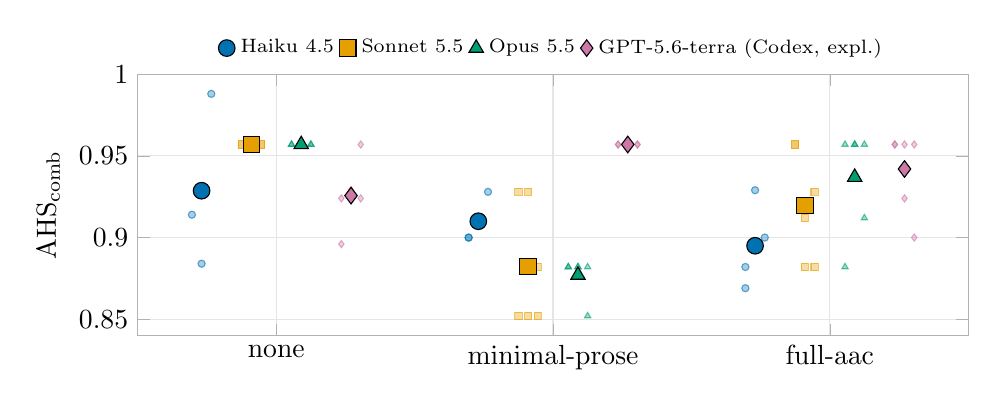
\begin{tikzpicture}
\begin{axis}[width=\linewidth, height=4.9cm, ymin=0.84, ymax=1.0, xmin=-0.5, xmax=2.5,
  xtick={0,1,2}, xticklabels={none, minimal-prose, full-aac}, ylabel={$\mathrm{AHS}_{\mathrm{comb}}$},
  ytick={0.85,0.90,0.95,1.00}, yticklabel style={/pgf/number format/fixed,/pgf/number format/precision=2},
  grid=major, grid style={gray!20}, axis line style={gray!60}, tick style={gray!60},
  legend style={font=\scriptsize, at={(0.5,1.02)}, anchor=south, legend columns=4, draw=none},
  every axis plot/.append style={only marks}]
\addplot[mark=*, mark size=1.3pt, draw=oiBlue, fill=oiBlue, fill opacity=0.35, draw opacity=0.6, forget plot]
  coordinates {(-0.305,0.914) (-0.270,0.884) (-0.235,0.988) (0.695,0.900) (0.730,0.912) (0.765,0.928) (0.695,0.900) (1.695,0.882) (1.730,0.929) (1.765,0.900) (1.695,0.869)};
\addplot[mark=*, mark size=3pt, draw=black, fill=oiBlue, line width=0.4pt]
  coordinates {(-0.270,0.9287) (0.730,0.9100) (1.730,0.8950)};
\addlegendentry{Haiku 4.5}
\addplot[mark=square*, mark size=1.3pt, draw=oiOrange, fill=oiOrange, fill opacity=0.35, draw opacity=0.6, forget plot]
  coordinates {(-0.125,0.957) (-0.090,0.957) (-0.055,0.957) (-0.125,0.957) (-0.090,0.957) (-0.055,0.957) (0.875,0.852) (0.910,0.852) (0.945,0.852) (0.875,0.928) (0.910,0.928) (0.945,0.882) (1.875,0.957) (1.910,0.912) (1.945,0.882) (1.875,0.957) (1.910,0.882) (1.945,0.928)};
\addplot[mark=square*, mark size=3pt, draw=black, fill=oiOrange, line width=0.4pt]
  coordinates {(-0.090,0.9570) (0.910,0.8823) (1.910,0.9197)};
\addlegendentry{Sonnet 5.5}
\addplot[mark=triangle*, mark size=1.3pt, draw=oiGreen, fill=oiGreen, fill opacity=0.35, draw opacity=0.6, forget plot]
  coordinates {(0.055,0.957) (0.090,0.957) (0.125,0.957) (0.055,0.957) (0.090,0.957) (0.125,0.957) (1.055,0.882) (1.090,0.882) (1.125,0.852) (1.055,0.882) (1.090,0.882) (1.125,0.882) (2.055,0.882) (2.090,0.957) (2.125,0.912) (2.055,0.957) (2.090,0.957) (2.125,0.957)};
\addplot[mark=triangle*, mark size=3pt, draw=black, fill=oiGreen, line width=0.4pt]
  coordinates {(0.090,0.9570) (1.090,0.8770) (2.090,0.9370)};
\addlegendentry{Opus 5.5}
\addplot[mark=diamond*, mark size=1.3pt, draw=oiPink, fill=oiPink, fill opacity=0.35, draw opacity=0.6, forget plot]
  coordinates {(0.235,0.896) (0.270,0.929) (0.305,0.924) (0.235,0.924) (0.270,0.924) (0.305,0.957) (1.235,0.957) (1.270,0.957) (1.305,0.957) (1.235,0.957) (1.270,0.957) (1.305,0.957) (2.235,0.957) (2.270,0.924) (2.305,0.957) (2.235,0.957) (2.270,0.957) (2.305,0.900)};
\addplot[mark=diamond*, mark size=3pt, draw=black, fill=oiPink, line width=0.4pt]
  coordinates {(0.270,0.9257) (1.270,0.9570) (2.270,0.9420)};
\addlegendentry{GPT-5.6-terra (Codex, expl.)}
\draw[gray!70, dashed] (axis cs:-0.5,0.80) -- (axis cs:2.5,0.80);
\end{axis}
\end{tikzpicture}
